\newcommand{\E}{\mathbb{E}}
\newcommand{\Rx}{\bm{R}_{x}}
\newcommand{\CC}{\bm{C\!C}}
\newcommand{\x}{\underline{x}}
\newcommand{\w}{\underline{w}}
\newcommand{\conv}{\operatorname{conv}}
\newcommand{\sv}{\sigma_v^2}
\newcommand{\Qf}{\operatorname{Q}}


%=====================================================================
\section{Partie 1.3 -- Filtre de Wiener et hyperplans séparateurs}
%=====================================================================

\subsection{Cadre et notations}
% Repli si le package bm n'est pas chargé dans le préambule.
\providecommand{\bm}[1]{\boldsymbol{#1}}
On reprend le modèle du sujet : $d(n)$ i.i.d.\ dans $\{+1,-1\}$ (donc $\bm{R}_d=\bm I$), bruit blanc gaussien $v(n)\sim\mathcal N(0,\sv)$, et
\begin{equation}
 \x(n)=\CC\,\bm D(n)+\underline v(n),\qquad
 \bm D(n)=[d(n),d(n-1),\dots,d(n-P-M+2)]^T ,
\end{equation}
avec $\CC\in\mathbb R^{P\times(P+M-1)}$ la matrice de convolution construite à partir de $\underline c=[c(0),\dots,c(M-1)]^T$. Les motifs non bruités de $\mathcal E^{+}$ (resp.\ $\mathcal E^{-}$) sont les $2^{P+M-2}$ vecteurs $\underline s=\CC\bm D$ obtenus pour $d(n)=+1$ (resp.\ $-1$). On les note $\mathcal S^{+}$ et $\mathcal S^{-}$. Les dimensions $M=\operatorname{length}(\underline c)$ et $P$ sont des paramètres du code, qui accepte donc n'importe quel $\underline c$.

\paragraph{Propriété de symétrie.} L'ensemble des symboles passés étant stable par changement de signe, $\mathcal S^{-}=-\mathcal S^{+}$. Tout ce qui suit en découle : les hyperplans séparateurs « raisonnables » passent par l'origine, et le TEB total est égal au TEB conditionnel à $d(n)=+1$.

\paragraph{RSB.} Avec $\bm R_d=\bm I$, $\;\mathrm{RSB}=10\log_{10}\!\big(\underline c^T\bm R_d\,\underline c/\sv\big)=10\log_{10}\!\big(\|\underline c\|^2/\sv\big)$. Pour $\underline c=[1,0.5]^T$, $\|\underline c\|^2=1{,}25$ et $\sv=0{,}01\,/\,0{,}2\,/\,1$ correspondent à $\approx 21{,}0\,/\,8{,}0\,/\,1{,}0$~dB.

\subsection{Calcul du filtre de Wiener}
On estime $d(n)$ (retard nul) par $y(n)=\w^T\x(n)$ en minimisant $J(\w)=\E[(d(n)-\w^T\x(n))^2]$. L'équation normale $\Rx\w=\bm p$ s'exprime ici en fonction de $\CC$ :
\begin{align}
 \Rx&=\E[\x\x^T]=\CC\bm R_d\CC^T+\sv\bm I=\CC\CC^T+\sv\bm I,\\
 \bm p&=\E[\x(n)d(n)]=\CC\,\bm e_1=[c(0),0,\dots,0]^T,\\
 \w_{\rm opt}&=\big(\CC\CC^T+\sv\bm I\big)^{-1}\bm p .
\end{align}
Pour $\underline c=[1,0.5]^T$ et $P=2$ :
$\CC=\begin{pmatrix}1&0.5&0\\0&1&0.5\end{pmatrix}$, $\;\Rx=\begin{pmatrix}1{,}25+\sv&0{,}5\\0{,}5&1{,}25+\sv\end{pmatrix}$ et donc
\begin{equation}
 \w_{\rm opt}=\frac{1}{(1{,}25+\sv)^2-0{,}25}\begin{pmatrix}1{,}25+\sv\\-0{,}5\end{pmatrix}.
\end{equation}
La décision est $\hat d(n)=\operatorname{sign}(\w_{\rm opt}^T\x(n))$ et l'\emph{hyperplan de Wiener} est $HP_{\rm Wiener}=\{\x\;|\;\w_{\rm opt}^T\x=0\}$ ; il passe par l'origine (symétrie des classes, pas de seuil nécessaire).

\begin{table}[H]\centering
\begin{tabular}{cccc}\toprule
$\sv$ & RSB (dB) & $\w_{\rm opt}$ & angle de la normale\\\midrule
0,01 & 20,97 & $[0{,}9420,\;-0{,}3738]^T$ & $-21{,}6^\circ$\\
0,2  & 7,96 & $[0{,}7827,\;-0{,}2699]^T$ & $-19{,}0^\circ$\\
1,0  & 0,97 & $[0{,}4675,\;-0{,}1039]^T$ & $-12{,}5^\circ$\\\bottomrule
\end{tabular}
\caption{Coefficients de Wiener pour $\underline c=[1,0.5]^T$, $P=2$ (le script \texttt{partie1\_3\_wiener\_hyperplans.m} vérifie aussi $\w_{\rm opt}$ par estimation empirique $\hat{\bm R}_x^{-1}\hat{\bm p}$).}
\end{table}

\paragraph{Comportement limite.}
Quand $\sv\to\infty$, $\w_{\rm opt}\propto\bm p\propto\bm e_1$ : c'est le filtre adapté, l'hyperplan tend vers $\{x(n)=0\}$ (angle $0^\circ$, d'où la tendance du tableau). Quand $\sv\to 0$, $\w_{\rm opt}\to(\CC\CC^T)^{-1}\CC\bm e_1$, soit $\w^T\CC=\bm e_1^T\bm\Pi$ avec $\bm\Pi$ le projecteur orthogonal sur l'espace-lignes de $\CC$ : c'est une inversion « zero-forcing » au sens des moindres carrés, qui ne peut pas annuler exactement l'interférence entre symboles puisque $P<P+M-1$.

\subsection{Hyperplan de Wiener, frontière de Bayes et optimalité}
La figure~\ref{fig:wb} superpose, pour trois variances, les nuages bruités, la frontière de Bayes $\partial\mathcal E=\{P_+=P_-\}$ (calculée sur une grille de $200\times200$ points) et l'hyperplan de Wiener.

\begin{figure}[H]\centering
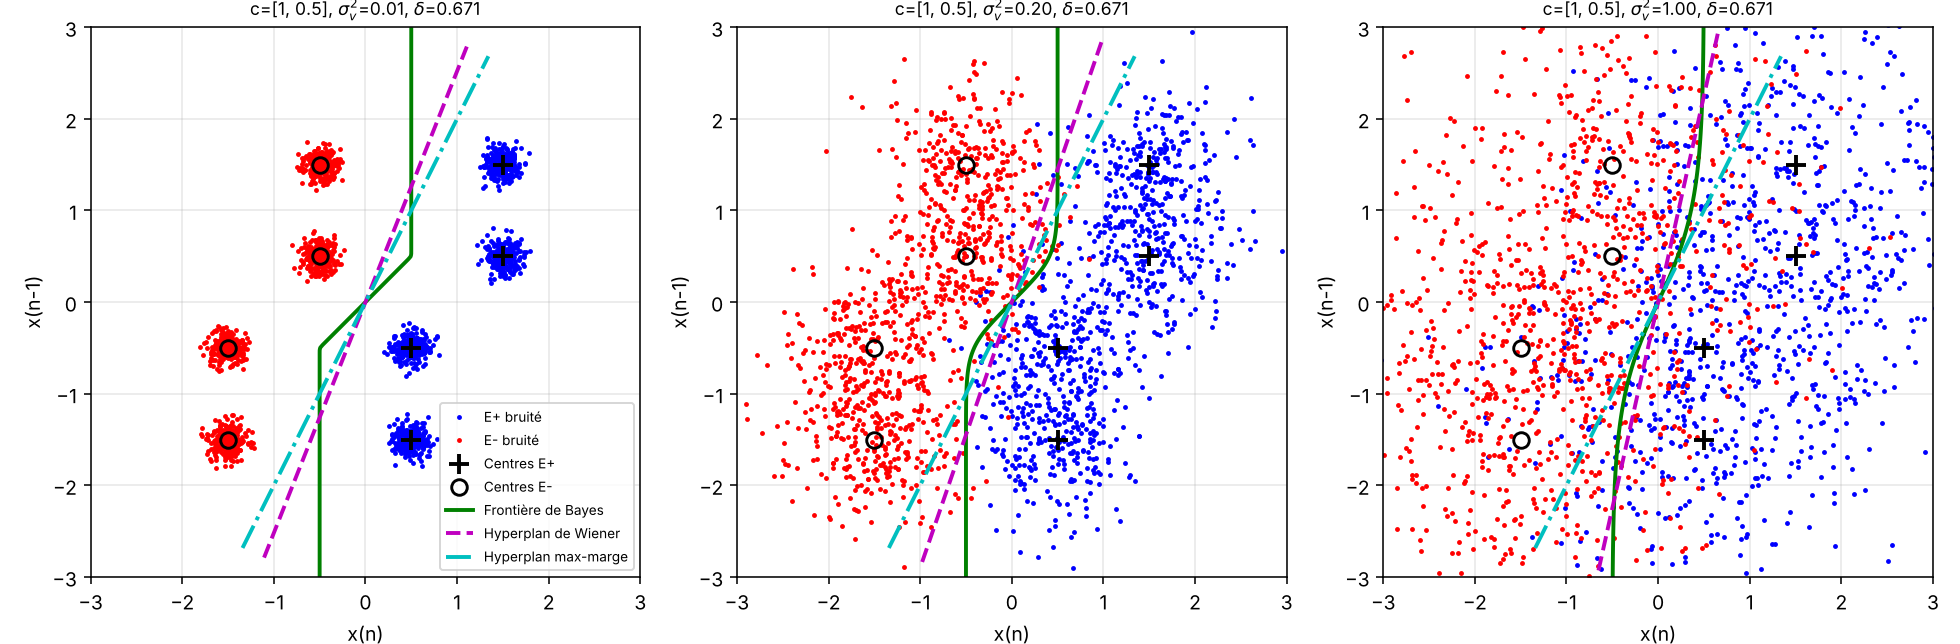
\includegraphics[width=\linewidth]{figures/fig1_wiener_bayes_sigma.png}
\caption{Frontière de Bayes (vert), hyperplan de Wiener (magenta, tirets) et hyperplan à marge maximale (cyan, section~\ref{sec:sep}) pour $\sv=0{,}01$, $0{,}2$ et $1$. Les classes sont linéairement séparables dans les trois cas (les motifs sont séparables ; c'est le bruit qui crée le recouvrement).}\label{fig:wb}
\end{figure}

\paragraph{Interprétation (optimalité).}
\begin{itemize}
 \item Le \textbf{classifieur bayésien MAP} minimise la probabilité d'erreur parmi \emph{tous} les classifieurs (linéaires ou non) : $\mathrm{TEB}_{\rm Bayes}\le\mathrm{TEB}$ de n'importe quelle autre règle. Sa frontière est \emph{non linéaire} : polygonale (médiatrices entre motifs voisins de classes opposées) quand $\sv$ est petit, de plus en plus lisse et proche d'une droite quand $\sv$ augmente.
 \item Le \textbf{filtre de Wiener} est optimal au sens de l'erreur quadratique moyenne \emph{parmi les filtres linéaires}, pas au sens du TEB. Il fournit un hyperplan, donc une frontière rectiligne.
 \item Quand $\sv$ est grand, la frontière de Bayes se linéarise (développement de $\ln P_+/P_-$ au premier ordre en $1/\sv$ : direction $\propto$ moyenne de $\mathcal S^+=c(0)\bm e_1$) et coïncide avec l'hyperplan de Wiener : à fort bruit, le Wiener est quasi optimal. À faible bruit et surtout à RSB moyen, la frontière de Bayes s'écarte de la droite et le classifieur bayésien gagne (figure~\ref{fig:teb}).
\end{itemize}

%---------------------------------------------------------------------
\subsection{Un meilleur hyperplan séparateur}\label{sec:sep}
%---------------------------------------------------------------------
\paragraph{Séparabilité linéaire et géométrie.}
Comme $\mathcal S^-=-\mathcal S^+$, un hyperplan affine $\w^T\x=b$ sépare les deux classes si $\w^T\underline s>|b|\ge 0$ pour tout $\underline s\in\mathcal S^+$ : le cas $b=0$ est donc toujours aussi bon que les autres.

\noindent\textbf{Proposition.} 
$\mathcal E^+$ et $\mathcal E^-$ sont linéairement séparables $\iff 0\notin\conv(\mathcal S^+)$. Dans ce cas, la marge maximale est $\delta=\operatorname{dist}(0,\conv\mathcal S^+)=\max_{\|\w\|=1}\min_{\underline s\in\mathcal S^+}\w^T\underline s$, atteinte pour $\w^\star\propto\underline x^\star$ où $\underline x^\star=\arg\min_{\underline x\in\conv\mathcal S^+}\|\underline x\|$ est le point de l'enveloppe convexe le plus proche de l'origine.
\noindent\emph{Idée de preuve.} C'est le théorème de séparation d'un point et d'un convexe fermé : le segment le plus court entre $0$ et $\conv\mathcal S^+$ est orthogonal à l'hyperplan séparateur de marge maximale ; pour tout $\w$ unitaire, $\min_s\w^T\underline s\le\w^T\underline x^\star\le\|\underline x^\star\|=\delta$, avec égalité pour $\w=\underline x^\star/\delta$. \hfill$\square$

\paragraph{Degré de séparabilité.} $\delta$ \emph{quantifie} la séparabilité linéaire : $\delta=0$ (origine dans l'enveloppe) $\Rightarrow$ non séparable ; plus $\delta$ est grand, plus la séparation est robuste. Le rapport $\rho=\delta/\sigma_v$ compare la marge à l'écart-type du bruit. Toute règle linéaire (donc Wiener) a une marge $\min_s\w^T\underline s/\|\w\|\le\delta$. Une condition \emph{suffisante} simple est $|c(0)|>\sum_{i\ge1}|c(i)|$ (l'œil de $x(n)$ seul est ouvert).

\paragraph{Méthode proposée (hyperplan à marge maximale par enveloppe convexe).}
Plutôt que d'appeler un solveur de SVM, on résout directement
\begin{equation}
 \min_{\bm\lambda}\ \|\bm S^+\bm\lambda\|^2\quad\text{s.c. }\ \bm\lambda\ge0,\ \ \bm 1^T\bm\lambda=1,
\end{equation}
où $\bm S^+$ rassemble les centres de $\mathcal E^+$ en colonnes. Il s'agit d'une projection de l'origine sur un polytope ; on l'implémente par un gradient projeté sur le simplexe (projection exacte par tri, pas $1/L$ avec $L=2\lambda_{\max}(\bm S^{+T}\bm S^+)$), sans toolbox (\texttt{hyperplan\_max\_marge.m}). Les centres $\underline s_i$ tels que $\lambda_i>0$ sont les « vecteurs de support ».

\paragraph{Exemple traité à la main ($\underline c=[1,0.5]^T$, $P=2$).} $\mathcal S^+=\{(1{,}5;1{,}5),(1{,}5;0{,}5),(0{,}5;-0{,}5),(0{,}5;-1{,}5)\}$ forme un parallélogramme. Le point le plus proche de $0$ est sur l'arête reliant $(0{,}5;-0{,}5)$ à $(1{,}5;1{,}5)$ (direction $(1,2)$) : $\underline x^\star=(0{,}6;-0{,}3)$, donc
\begin{equation}
 \delta=\sqrt{0{,}45}=\tfrac{3}{\sqrt{20}}\approx0{,}6708,\qquad \w^\star\propto(2,-1)\ \ (\text{angle }-26{,}6^\circ).
\end{equation}
C'est exactement ce que renvoie le code (figure~\ref{fig:geo}). La marge de Wiener vaut seulement $0{,}6492$, $0{,}6357$, $0{,}5966$ pour $\sv=0{,}01,\,0{,}2,\,1$.

\begin{figure}[H]\centering
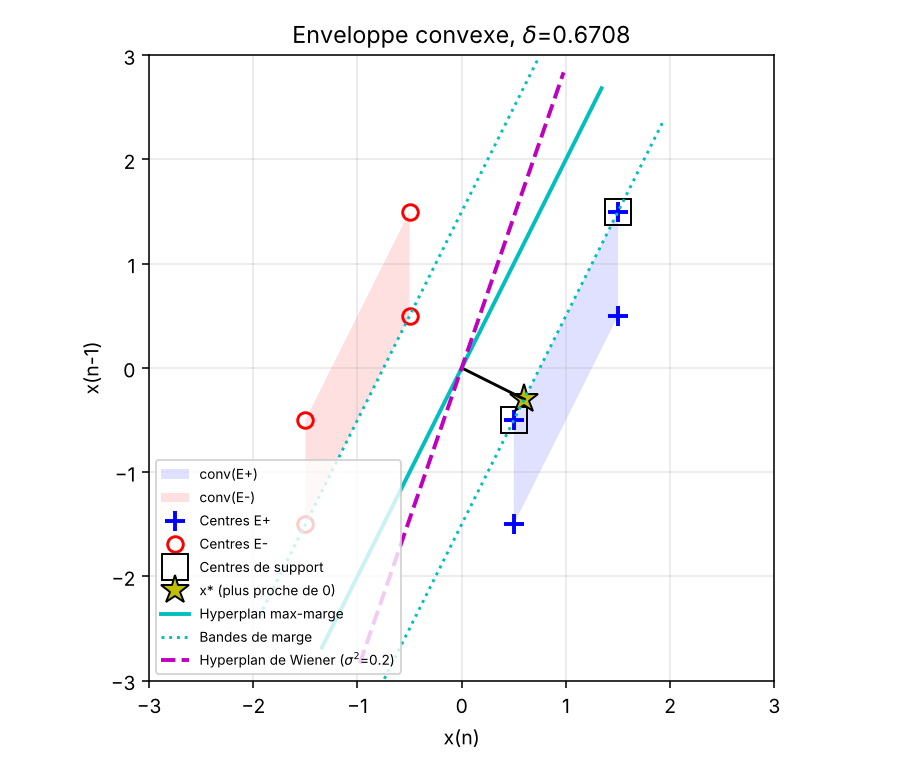
\includegraphics[width=0.62\linewidth]{figures/fig2_hyperplans_comparaison.png}
\caption{Enveloppes convexes de $\mathcal S^+$ et $\mathcal S^-$, point $\underline x^\star$, centres de support, hyperplan à marge maximale (bandes de marge en pointillés) et hyperplan de Wiener ($\sv=0{,}2$).}\label{fig:geo}
\end{figure}

\paragraph{Critère alternatif : hyperplan de TEB minimal.}
La marge maximale ne regarde que le pire cas. Comme le bruit est gaussien, le TEB exact d'une règle linéaire $\operatorname{sign}(\w^T\x)$ est connu en forme fermée :
\begin{equation}
 \mathrm{TEB}(\w)=\frac1{2^{P+M-2}}\sum_{\underline s\in\mathcal S^+}\Qf\!\Big(\frac{\w^T\underline s}{\sigma_v\|\w\|}\Big),\qquad \Qf(u)=\tfrac12\operatorname{erfc}(u/\sqrt2).
\end{equation}
On minimise cette fonction (\texttt{fminsearch}, initialisée en Wiener et en max-marge) : \texttt{hyperplan\_min\_teb.m}. On obtient le meilleur classifieur linéaire \emph{pour ce $\sv$}. Deux cas limites éclairants : pour $\sv\to0$, la somme est dominée par le terme de plus petite marge et l'on retrouve l'hyperplan à marge maximale ; pour $\sv\to\infty$, $\Qf(u)\approx\frac12-\frac u{\sqrt{2\pi}}$ et l'on retrouve le filtre adapté $\w\propto\E[\x\,|\,d=+1]=c(0)\bm e_1$.

\paragraph{Comparaison.}
\begin{table}[H]\centering\small
\begin{tabular}{ccccccc}\toprule
 & & \multicolumn{2}{c}{marge $\min_s\w^T s/\|\w\|$} & \multicolumn{3}{c}{TEB théorique}\\\cmidrule(lr){3-4}\cmidrule(lr){5-7}
$\sv$ & $\rho=\delta/\sigma_v$ & Wiener & Max-marge & Wiener & Max-marge & Min-TEB\\\midrule
0,01 & 6,71 & 0,6492 & \textbf{0,6708} & $1{,}06\!\cdot\!10^{-11}$ & $4{,}93\!\cdot\!10^{-12}$ & $\mathbf{3{,}41\!\cdot\!10^{-12}}$\\
0,2  & 1,50 & 0,6357 & \textbf{0,6708} & $\mathbf{2{,}87\!\cdot\!10^{-2}}$ & $3{,}65\!\cdot\!10^{-2}$ & $\mathbf{2{,}87\!\cdot\!10^{-2}}$\\
1,0  & 0,67 & 0,5966 & \textbf{0,6708} & $\mathbf{1{,}75\!\cdot\!10^{-1}}$ & $1{,}92\!\cdot\!10^{-1}$ & $\mathbf{1{,}75\!\cdot\!10^{-1}}$\\\bottomrule
\end{tabular}
\caption{$\underline c=[1,0.5]^T$, $P=2$. Le max-marge a toujours la plus grande marge, mais sa supériorité en TEB n'apparaît qu'à très fort RSB.}\label{tab:cmp}
\end{table}

\paragraph{Lecture honnête du résultat.} Le hyperplan à marge maximale est « meilleur » au sens géométrique (marge $+3\,\%$ à $+12\,\%$ par rapport à Wiener) et au sens du TEB \emph{asymptotique} : il devient meilleur que Wiener à partir d'environ 18~dB pour $\underline c=[1,0.5]^T$ (TEB théorique $\approx5\cdot10^{-7}$, donc non observable avec $N=10^4$ échantillons) et 19~dB pour $\underline c=[1,0.5,0.2]^T$. Pour des RSB usuels, Wiener est \emph{déjà quasi optimal parmi les hyperplans} (le min-TEB lui est identique à 3 chiffres pour $\sv\ge0{,}2$), car le critère EQM tient compte de la dispersion de tous les motifs et pas seulement du plus proche. Le seul séparateur nettement meilleur en moyenne est le classifieur \emph{non linéaire} de Bayes.

%---------------------------------------------------------------------
\subsection{RSB et taux d'erreur binaire}
%---------------------------------------------------------------------
Pour chaque RSB de $0$ à $20$~dB on fixe $\sv=\|\underline c\|^2/10^{\mathrm{RSB}/10}$, on simule $N=10^5$ observations et on mesure $\mathrm{TEB}=\frac1N\sum_n\mathbb 1[\hat d(n)\neq d(n)]$ pour : le classifieur MAP de Bayes, le filtre de Wiener, l'hyperplan à marge maximale et l'hyperplan à TEB minimal.

\begin{figure}[H]\centering
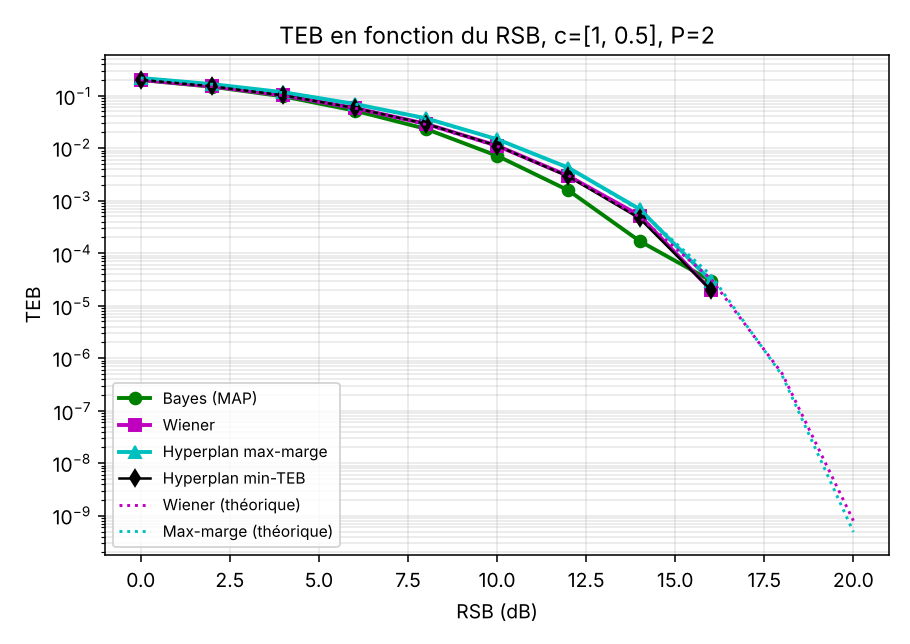
\includegraphics[width=0.75\linewidth]{figures/fig3_teb_rsb.png}
\caption{TEB en fonction du RSB ($\underline c=[1,0.5]^T$, $P=2$). Pointillés : TEB théorique des règles linéaires. Les points à TEB nul sur $10^5$ essais ne sont pas tracés.}\label{fig:teb}
\end{figure}

\begin{table}[H]\centering
\begin{tabular}{rcccc}\toprule
RSB (dB) & Bayes & Wiener & Max-marge & Min-TEB\\\midrule
0  & 0,1982 & 0,1994 & 0,2165 & 0,1995\\
4  & 0,0967 & 0,1009 & 0,1160 & 0,1009\\
8  & 0,0233 & 0,0290 & 0,0370 & 0,0290\\
10 & 0,0072 & 0,0111 & 0,0148 & 0,0111\\
12 & 0,0016 & 0,0030 & 0,0042 & 0,0029\\
14 & 0,00017 & 0,00052 & 0,00069 & 0,00046\\\bottomrule
\end{tabular}
\caption{TEB simulé ($N=10^5$, graine fixée). Les valeurs exactes dépendent de la graine du générateur.}
\end{table}

\paragraph{Interprétation.} (i) À RSB faible, les trois règles se rejoignent (frontière de Bayes quasi linéaire). (ii) À RSB moyen/élevé, Bayes réduit le TEB d'un facteur $\approx 1{,}5$ à $3$ par rapport à Wiener (ex.\ $0{,}0072$ contre $0{,}0111$ à 10~dB) : c'est le gain d'une frontière non linéaire. (iii) L'hyperplan min-TEB ne gagne presque rien sur Wiener, ce qui confirme que Wiener est proche du meilleur séparateur \emph{linéaire}. (iv) L'hyperplan max-marge est le moins bon sur la plage $0$--$14$~dB (il ignore le bruit moyen) : maximiser la marge est un critère de pire cas, pertinent uniquement quand $\sv$ est très faible.

%---------------------------------------------------------------------
\subsection{Influence du canal $\underline c$}
%---------------------------------------------------------------------
\begin{table}[H]\centering\small
\begin{tabular}{lccccccc}\toprule
$\underline c$ & $P$ & $\delta$ & sép.\ lin. & marge W & Bayes & Wiener & Max-marge\\\midrule
$[1,\ 0.5]$ & 2 & 0,671 & oui & 0,641 & 0,0072 & 0,0105 & 0,0143\\
$[1,\ 0.9]$ & 2 & 0,141 & oui (faible) & 0,132 & 0,0996 & 0,1037 & 0,1887\\
$[0.5,\ 1]$ & 2 & 0 & \textbf{non} & $<0$ & 0,0965 & 0,3541 & --\\
$[1,\ -0.5]$ & 2 & 0,671 & oui & 0,641 & 0,0073 & 0,0107 & 0,0142\\
$[1,\ 0.5,\ 0.2]$ & 3 & 0,818 & oui & 0,770 & 0,0033 & 0,0066 & 0,0070\\
$[0.4048,\ 0.8164,\ 0.4084]$ & 3 & 0 & \textbf{non} & $<0$ & 0,1560 & 0,2942 & --\\\bottomrule
\end{tabular}
\caption{TEB simulés à RSB $=10$~dB ($N=5\cdot10^4$, $P=M$). « marge W » : marge de l'hyperplan de Wiener (négative = des motifs mal classés même sans bruit).}\label{tab:canaux}
\end{table}

\begin{figure}[H]\centering
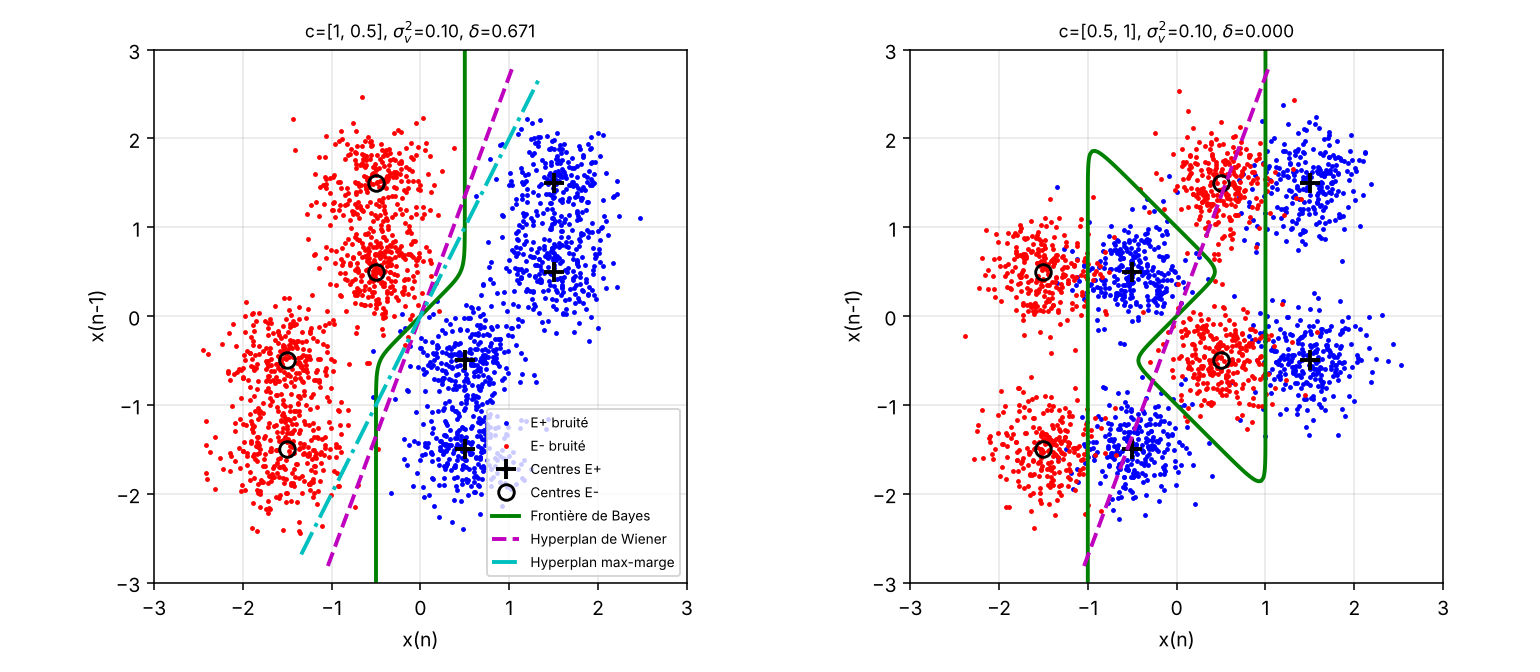
\includegraphics[width=0.9\linewidth]{figures/fig4_separable_vs_non_separable.png}
\caption{Gauche : $\underline c=[1,0.5]^T$ (séparable). Droite : $\underline c=[0.5,1]^T$ : $c(0)<c(1)$, les enveloppes convexes se recouvrent, aucun hyperplan ne sépare les classes, même sans bruit ; la frontière de Bayes devient fortement non linéaire.}
\end{figure}

\paragraph{Observations.}
\begin{itemize}
 \item Changer le signe de $c(1)$ ne modifie pas $\delta$ (symétrie des symboles), seulement l'orientation de l'hyperplan.
 \item La séparabilité est gouvernée par le rapport entre $c(0)$ et l'interférence : $[1,0.9]$ est à peine séparable ($\delta=0{,}14$) ; le max-marge, qui ne tient compte que de cette marge minuscule, dégrade fortement le TEB ($0{,}19$) alors que Wiener reste proche de Bayes.
 \item Si $c(0)<c(1)$ (canal à retard ou à phase non minimale), les classes ne sont plus séparables linéairement avec un retard nul : Wiener échoue ($\mathrm{TEB}\approx0{,}35$ pour $[0.5,1]$, quasi aléatoire) alors que Bayes garde $0{,}097$ grâce à sa frontière non linéaire. L'information sur $d(n)$ est surtout portée par $x(n+1)$ ; un filtre linéaire avec retard (non demandé) corrigerait en partie ce défaut.
 \item $\delta$ augmente avec la taille de l'observation ($0{,}671\to0{,}818\to0{,}871$ pour $(M,P)=(2,2),(3,3),(5,5)$ avec les canaux testés) : plus de coordonnées $\Rightarrow$ plus d'information.
\end{itemize}

%---------------------------------------------------------------------
\subsection{Montée en dimension : $M=3$ puis $M>3$}
%---------------------------------------------------------------------
Pour $\underline c=[1,0.5,0.2]^T$, $P=3$, les $16$ motifs de chaque classe vivent en 3D (figure~\ref{fig:3d}) ; les hyperplans sont des plans, tracés à partir d'une base orthonormée du plan ($\texttt{null}(\w^T)$) pour éviter toute division par une petite composante. Ici $\delta=0{,}818$ et la marge de Wiener ($\mathrm{RSB}=10$~dB) vaut $0{,}770$.

\begin{figure}[H]\centering
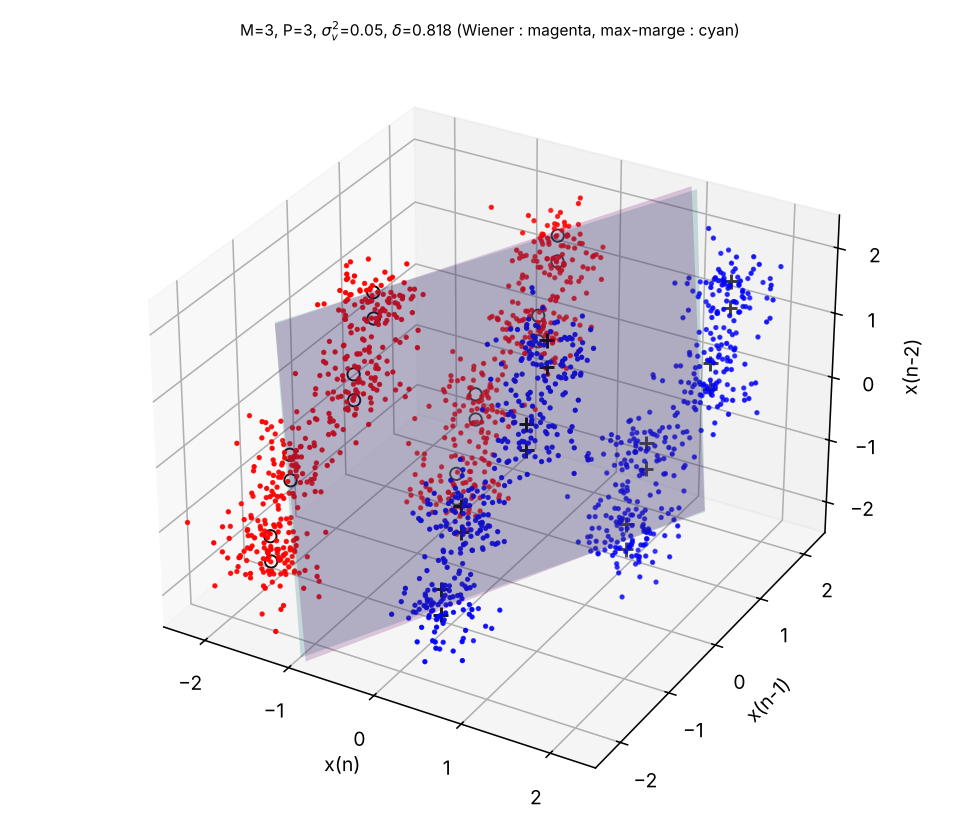
\includegraphics[width=0.62\linewidth]{figures/fig5_3D_M3.png}
\caption{$M=P=3$, $\sv=0{,}05$ : nuages bruités, motifs, plan de Wiener (magenta) et plan à marge maximale (cyan).}\label{fig:3d}
\end{figure}

Pour $M>3$, on utilise t-SNE (\texttt{tsne} de MATLAB, repli sur l'ACP si la toolbox est absente) sur un échantillon d'observations \emph{et} sur les centres non bruités, pour $\underline c=[1,0.5,0.2,0.1,0.05]^T$, $P=5$ (figure~\ref{fig:tsne}). Les classes sont toujours linéairement séparables ($\delta=0{,}871$, marge de Wiener $0{,}829$), et à $\mathrm{RSB}=10$~dB : $\mathrm{TEB}_{\rm Bayes}=0{,}0035$, $\mathrm{TEB}_{\rm Wiener}=0{,}0066$, $\mathrm{TEB}_{\rm max\text{-}marge}=0{,}0073$.

\begin{figure}[H]\centering
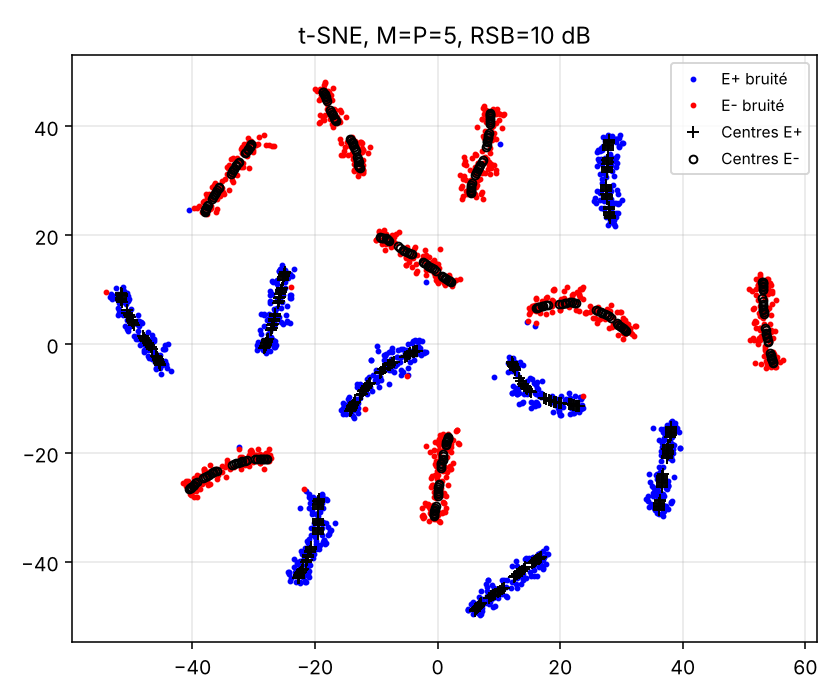
\includegraphics[width=0.55\linewidth]{figures/fig6_tsne_M5.png}
\caption{Projection t-SNE ($P=5$, RSB $=10$~dB).}\label{fig:tsne}
\end{figure}
\noindent\textbf{Précaution.} t-SNE ne conserve ni les distances ni la rectilinéarité : la séparation visible en 2D est seulement qualitative. La séparabilité linéaire doit être jugée dans l'espace d'origine, par $\delta$ (ou la marge de Wiener), comme fait ci-dessus.

%=====================================================================
\section*{Fichiers fournis}
%=====================================================================
\begin{itemize}\small
 \item \texttt{matlab/partie1\_3\_wiener\_hyperplans.m} : script principal (sections 1 à 7) ; fonctions : \texttt{centres\_classes}, \texttt{generer\_observations}, \texttt{filtre\_wiener}, \texttt{classifieur\_bayes}, \texttt{hyperplan\_max\_marge}, \texttt{hyperplan\_min\_teb}, \texttt{teb\_lineaire\_theorique}, \texttt{tracer\_classes\_2D}, \texttt{tracer\_classes\_3D}.
 \item \texttt{python/diffwave\_test.py} (+ \texttt{requirements.txt}) : test du modèle DiffWave pré-entraîné.
\end{itemize}

